\documentclass{article}

\usepackage{cancel}
\usepackage{tikz}
\usepackage{amsmath}
\usepackage{geometry}
\usepackage{graphicx}
\usepackage{amsfonts} 
\usepackage{verbatim}
\usepackage{mathrsfs}  
\usepackage{lmodern}
\usepackage{braket}
\usepackage{hyperref}

\hypersetup{
    colorlinks=true,
    linkcolor=black,
}

\renewcommand{\contentsname}{Indice}

\tikzset{sum/.style= {draw, fill=white, very thick, circle, node distance=0.5cm}}
\numberwithin{equation}{subsection}

\title{Appunti di Elettrotecnica ed Elettronica}
\author{Giacomo Sturm}
\date{AA: 2023/2024 - Ing. Informatica}

\begin{document}

\maketitle

\vspace{10mm}

\begin{center}
    Sorgente del file LaTeX disponibile su \url{https://github.com/00Darxk/Elettrotecnica-ed-Elettronica}
\end{center}

\clearpage

\tableofcontents

\clearpage

\section{Introduzione: Elementi di Fisica}

\subsection{Forza Elettrica}
Le prime analisi documentate sugli effetti elettrici risalgono agli antichi greci, da cui deriva il nome "electron"; $\eta\lambda\varepsilon\kappa\tau\rho o\nu$ in greco. Letteralmente significa ambra, poiché 
quando viene sfregata contro della lana, è capace di attrarre materiali, ovvero è in grado di generare un campo elettrico.

La forza elettrica venne analizzata da Coulomb in maniera simile all'analisi di Newton sulla gravità, poiché le due forze presentano dei comportamenti simili. La forza di 
gravità è una forza attrattiva tra due masse nello spazio, per cui sono presenti due forze applicate ad entrambe le masse di modulo e direzione uguale, ma verso opposto: 
\begin{equation*}
    \vec{F}_{1\to2}=G\displaystyle\frac{m_1m_2}{r^2}\hat{r}_{1\to2}=-\vec{F}_{2\to1}
\end{equation*}
Analogamente la forza elettrica è presente solo nell'interazione tra due elementi dotati di una carica che può presentarsi in due classi diverse, per convezione 
positiva o negativa, vengono misurate in Coulomb $C$ nel SI. Due cariche appartenenti alla stessa classe si oppongono, mentre due cariche appartenenti a due classi diverse 
si attraggono:
\begin{gather}
    \vec{F}_{1\to2}=-k_0\displaystyle\frac{q_1q_2}{r^2}\hat{r}_{1\to2}=-\vec{F}_{2\to1}\\
    F=k_0\displaystyle\frac{|q_1q_2|}{r^2}
\end{gather} 
Viene chiamata $k_0$ costante elettrica nel vuoto. 


La forza di gravità è una forza solamente attrattiva e presenta una sola classe di masse a differenza della forza elettrica. Poiché la forza di gravità si 
presenta solamente dall'interazione tra due masse, una massa singola nello spazio non è soggetta a forze di gravità. Questa massa è pronta ad interagire con un eventuale 
seconda massa per comunicare tra di loro la massa deforma in qualche modo lo spazio. Convenzionalmente si considera una deformazione convessa nella zona di spazio dove 
si trova la massa: 
\begin{center}
    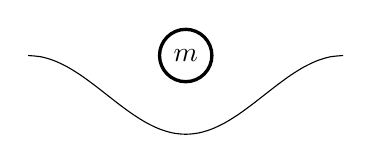
\begin{tikzpicture}[scale=2]
        \node[sum](o)at(0,0){$m$};
        \draw[-]plot[smooth, domain=-1:1](\x,{0.25*cos(180*(\x)-pi r)-0.25});
    \end{tikzpicture}
\end{center}

Poiché le cariche possono appartenere a due classi diverse per convenzione una carica positiva crea una deformazione concava, mentre una negativa una deformarzione convessa: 
\begin{center}
    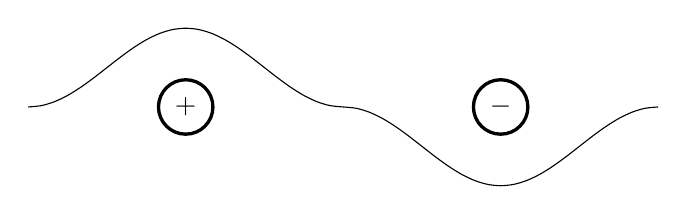
\begin{tikzpicture}[scale=2]
        \node[sum](o1)at(0,0){$+$};
        \draw[-]plot[smooth, domain=-1:1](\x,{-0.25*cos(180*(\x)-pi r)+0.25});
        
        \node[sum](o2)at(2,0){$-$};
        \draw[-]plot[smooth, domain=1:3](\x,{0.25*cos(180*(\x-2)-pi r)-0.25});
    \end{tikzpicture}
\end{center}
Per cui le cariche positive tendono a "scendere", mentre le cariche negative tendono a "salire". La deformazione spaziale è dovuta ad un campo gravitazionale o elettrico, 
dalle interazione del campo si genera una forza gravitazionale o elettrica. 

\subsection{Campo Elettrico}
Un campo elettrico $\vec{E}(x,y,z)$ è un campo vettoriale, ovvero è un insieme di vettori per ogni punto dello spazio dipendenti dalla loro posizione. Per misurare il campo 
generato da una carica $Q$ positiva per convenzione, si considera un'altra carica positiva $q<<Q$ usata per misurare la forza elettrica $\vec{F}$ generata dall'interazione con 
il campo $\vec{E}$. Si considera invece della costante elettrica nel vuoto $k_0$, la costante di permettività dielettrica nel vuoto $\varepsilon$:
\begin{gather}
    k_0=\displaystyle\frac{1}{4\pi\varepsilon_0},\:
    \varepsilon_0\approx8.86\times10^{-12}\left[\displaystyle\frac{C^2}{m^2}\frac{1}{N}\right]
\end{gather} 
Per misurare il campo elettrico in punto dello spazio di posizione $\vec{r}$ si considera la forza per unità di carica in quel punto:
\begin{equation}
    \vec{E}(x,y,z)=\displaystyle\frac{\vec{F}(x,y,z)}{q}=\frac{1}{4\pi\varepsilon_0}\frac{Q}{r^2}\hat{r}\left[\frac{N}{C}\right]
\end{equation}
Il campo elettrico generato da una singola carica puntiforme ha una direzione radiale e verso entrante se è una carica negativa ed uscente se si tratta di una carica positiva. 
Per indicare la direzione ed il verso di un campo vettoriale vengono usate linee di forza, la cui tangente in un punto rappresenta la direzione ed il verso del campo nello 
stesso punto. 
\begin{center}
    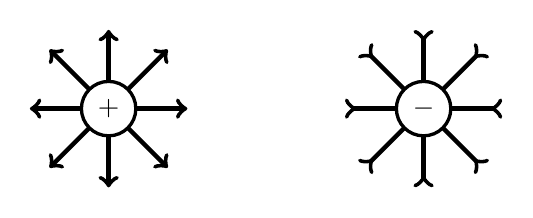
\begin{tikzpicture}[scale=2]
        \draw[<->, ultra thick](-0.5,0)--(0.5,0);
        \draw[>-<, ultra thick](1.5,0)--(2.5,0);

        \draw[<->, ultra thick](0,-0.5)--(0,0.5);
        \draw[>-<, ultra thick](2,-0.5)--(2,0.5);

        \draw[<->, ultra thick](-0.375,-0.375)--(0.375,0.375);
        \draw[<->, ultra thick](0.375,-0.375)--(-0.375,0.375);

        \draw[>-<, ultra thick](1.625,-0.375)--(2.375,0.375);
        \draw[>-<, ultra thick](2.375,-0.375)--(1.625,0.375);

        \node[sum](+)at(0,0){$+$};
        \node[sum](-)at(2,0){$-$};
    \end{tikzpicture}
\end{center}


In generale una forza elettrica è effetto dall'interazione di una carica $q$ con un campo elettrico $\vec{E}$, indipendentemente da ciò che genera il campo elettrico. Nel 
caso di una carica stazionaria o in moto rettilineo uniforme, si considera un campo elettro-stazionario, per cui la forza generata si esprime come il prodotto per la carica 
ed il campo elettrico: 
\begin{equation}
    \vec{F}=q\vec{E}
\end{equation}

L'unità di misura fondamentale usata per analizzare fenomeni elettrici nel SI è l'Ampere $A$, intensità di corrente, che ha sostituito il Coulomb $C$, unità di carica, 
entrambe sono cognomi di scienziati che hanno studiato l'elettricità, a differenza delle restanti grandezze fondamentali. Ciò spiega come non fosse chiaramanete 
idefntificabile la causa dei fenomeni elettrici in passato. 


In caso sia presente più di una carica stazionaria nel vuoto, per determinare il campo elettrico in un dato punto si considera il principio di sovrapposizione degli effetti 
(P.S.E.), applicabile solo in situazioni di tipo lineare, come nel vuoto essendo un elemento lineare. Per il principio della sovrapposizione degli effetti, il campo in un 
punto è dato dalla somma vettoriale di tutti i campi in quel punto, per cui i campi agiscono indipendentemente l'uno dall'altro. In una configurazione a due cariche, una 
positiva ed una negativa, il campo totale agente su una carica positiva posta in una posizione $P$ risulta essere: $\vec{E}_P=\vec{E}_1+\vec{E}_2$. 
\begin{center}
    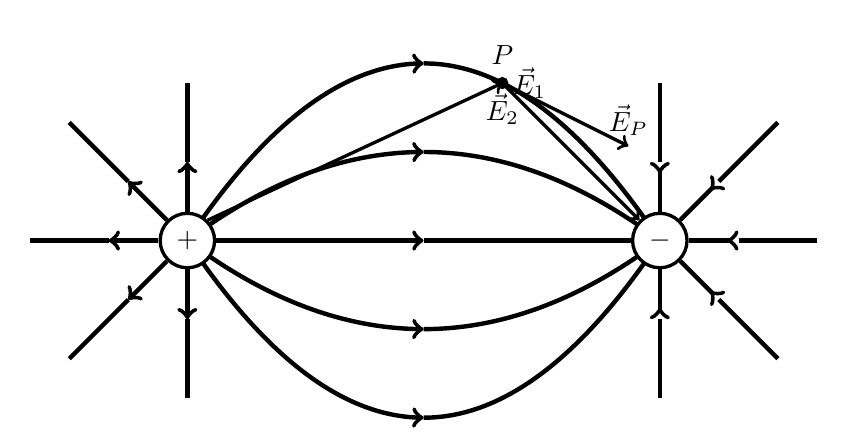
\begin{tikzpicture}[scale=2]
        \draw[->,ultra thick]plot[smooth, domain=0:1.5](\x,{0.25*(\x)*(\x-3)});
        \draw[-,ultra thick]plot[smooth, domain=1.5:3](\x,{(0.25*\x)*(\x-3)});

        \draw[->,ultra thick]plot[smooth, domain=0:1.5](\x,{-0.25*(\x)*(\x-3)});
        \draw[-,ultra thick]plot[smooth, domain=1.5:3](\x,{-0.25*(\x)*(\x-3)});

        \draw[->,ultra thick]plot[smooth, domain=0:1.5](\x,{0.5*(\x)*(\x-3)});
        \draw[-,ultra thick]plot[smooth, domain=1.5:3](\x,{(0.5*\x)*(\x-3)});

        \draw[->,ultra thick]plot[smooth, domain=0:1.5](\x,{-0.5*(\x)*(\x-3)});
        \draw[-,ultra thick]plot[smooth, domain=1.5:3](\x,{-0.5*(\x)*(\x-3)});

        \draw[<->,ultra thick](0,-0.5)--(0,0.5);
        \draw[ultra thick](0,-0.5)--(0,-1);
        \draw[ultra thick](0,0.5)--(0,1);

        \draw[>-<,ultra thick](3,-0.5)--(3,0.5);
        \draw[ultra thick](3,-0.5)--(3,-1);
        \draw[ultra thick](3,0.5)--(3,1);        

        \node[sum](+)at(0,0){$+$};
        \node[sum](-)at(3,0){$-$};

        \filldraw[circle](2,1)node[above]{$P$}circle(1pt);
        \draw[->,very thick](+.45)--(2,1)node[below]{$\vec{E}_2$};
        \draw[->,very thick](2,1)node[right]{$\vec{E}_1$}--(-.135);
        \draw[->,very thick](2,1)--(2.8,0.6)node[above]{$\vec{E}_P$};

        \draw[->, ultra thick](+.0)--(1.5,0);
        \draw[-,ultra thick](1.5,0)--(-.180);

        \draw[->,ultra thick](+.180)--(-0.5,0);
        \draw[ultra thick](-0.5,0)--(-1,0);
        \draw[-<,ultra thick](-.0)--(3.5,0);
        \draw[ultra thick](3.5,0)--(4,0);

        \draw[->,ultra thick](+.135)--(-0.375,0.375);
        \draw[->,ultra thick](+.225)--(-0.375,-0.375);
        \draw[-,ultra thick](-0.375,0.375)--(-0.75,0.75);
        \draw[-,ultra thick](-0.375,-0.375)--(-0.75,-0.75);

        \draw[-<,ultra thick](-.45)--(3.375,0.375);
        \draw[-<,ultra thick](-.315)--(3.375,-0.375);
        \draw[-,ultra thick](3.375,0.375)--(3.75,0.75);
        \draw[-,ultra thick](3.375,-0.375)--(3.75,-0.75);
    \end{tikzpicture}
\end{center}


Il campo elettrico stazionario, come il campo gravitazionale, è conservativo, per cui il lavoro svolto equivale all'opposto della differenza di energia potenziale. Per 
convenzione lo stato di riferimento dell'energia potenziale elettrica si trova ad una distanza infinita dalla carica, per cui l'energia corrisponde al lavoro necessario per 
spostare una carica $q$ da una distanza infinita ad una distanza finita $R$ da un campo elettrico $\vec{E}$. Si considera una campo elettrico generato da una carica puntiforme 
$Q$:
\begin{gather*}
    \Delta U(r)=-L=-\displaystyle\int_{+\infty}^R\vec{F}\cdot d\vec{r}\\
    \displaystyle\int_{+\infty}^Rq\vec{E}\cdot d\vec{r}=\int_{+\infty}^R\frac{1}{4\pi\varepsilon_0}\frac{qQ}{r^2}\cancelto{1}{\hat{r}\cdot \hat{r}}dr\\
    \cancelto{0}{-\displaystyle\frac{1}{4\pi\varepsilon_0}\frac{qQ}{+\infty}}+\frac{1}{4\pi\varepsilon_0}\frac{qQ}{R}
\end{gather*}
\begin{equation}
    U(r)=\frac{1}{4\pi\varepsilon_0}\frac{qQ}{R}=-L(r)
\end{equation}


Viene definito il potenziale elettrico $V$ il lavoro per unità di carica, viene misurato nel SI in Volt $V$:
\begin{equation}
    \Delta V=\displaystyle-\frac{L}{q}=-\int\frac{\vec{F}}{q}\cdot d\vec{r}=-\int\vec{E}\cdot d\vec{r}
\end{equation}
Corrisponde ad un integrale di linea del campo elettrico $\vec{E}$. 
Per un campo elettrico stazionario generato da una carica puntiforme $Q$ corrisponde a:
\begin{equation}
    V=\displaystyle\frac{1}{4\pi\varepsilon_0}\frac{Q}{R}\:\left[V\right]=\left[\frac{mN}{C}\right]
\end{equation}

In forma differenziale, il potenziale elettrico corrisponde a:
\begin{equation*}
    dV=-\vec{E}\cdot d\vec{r}=-(E_xdx+E_ydy+E_zdz)
\end{equation*}
Il differenziale $dV$ è un differenziale totale di un campo scalare $V(x,y,z)$, per cui corrisponde alla somma delle variazioni su ogni coordinata del differenziale della stessa: 
\begin{equation*}
    dV=\displaystyle\frac{\partial V}{\partial x}dx+\frac{\partial V}{\partial y}dy+\frac{\partial V}{\partial z}dz
\end{equation*}
Per il principio di indentità dei polinomi risulta:
\begin{equation*}
    \displaystyle\frac{\partial V}{\partial x}=-E_x,\:\frac{\partial V}{\partial y}=-E_y,\:\frac{\partial V}{\partial z}=-E_z
\end{equation*}

Si considera l'operatore differenziale vettoriale nabla: 
\begin{equation*}
    \vec{\nabla}:=\left(\displaystyle\frac{\partial}{\partial x},\,\frac{\partial}{\partial y},\,\frac{\partial}{\partial z}\right)
\end{equation*}
Per cui è possibile esprimere la relazione tra il potenziale elettrico ed il campo elettrico considerando l'operazione di gradiente su un campo scalare $\vec{\nabla}V$: 
\begin{equation}
    \vec{E}=-\vec{\nabla}V
\end{equation}

\end{document}